\documentclass{article}
\usepackage[utf8]{inputenc}
\usepackage[dvipsnames]{xcolor}
\usepackage[a4paper, total={6in, 10in}]{geometry}
\usepackage{graphicx}
\graphicspath{ {./images/} }

\title{Monads}
\author{dannymaate}
\date{11 July 2022}

\begin{document}
\maketitle

\section{Monads}
The infix operator \textcolor{Emerald}{\texttt{>>=}} is called \textcolor{Mulberry}{bind}. It is used to extract contents from a monad, e.g. we can reach inside \textcolor{Emerald}{\texttt{Just x}} to operate on \textcolor{Emerald}{\texttt{x}}.


\begin{verbatim}
instance Monad Maybe where
    -- (>>=) :: Maybe a -> (a -> Maybe b) -> Maybe b
    (Just x) >>= k      = k x
    Nothing  >>= _      = Nothing
    return              = pure
\end{verbatim}
The following are equivalent:
\begin{verbatim}
madd mx my =                            madd mx my = do
    mx >>= \x ->                            x <- mx 
    my >>= \y ->                            y <- my 
    return $ x + y                          return $ x + y
\end{verbatim}
\paragraph{Monad Laws}
\begin{enumerate}
    \item \texttt{return x >>= f    = f x} \textcolor{Mulberry}{\emph{Left identity}}
    \item \texttt{mx >>= return     = m x}
    \textcolor{Mulberry}{\emph{Right identity}}
    \item \texttt{(mx >>= f) >>= g  = mx >>= (\textbackslash x -> f x >>= g)} \textcolor{Mulberry}{\emph{Associativity}}
\end{enumerate}

\section{The State Monad}
A \emph{state transformer} takes an input state as its argument and produces an output state as its result.

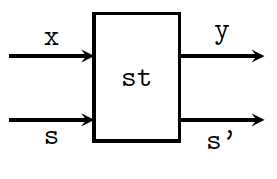
\includegraphics[scale=0.5]{images/st.PNG}
\begin{verbatim}
instant Monad ST where 
    -- (>>=) :: ST a -> (a -> ST b) -> ST b
    st >>= f = S(\ S ->
        let 
            (x, s') = app st s 
        in 
            app (f x) s')
\end{verbatim}

\



\end{document}